\documentclass{beamer}
\let\vec\mathbf
\mode<presentation>
\usepackage{amsmath}
\usepackage{amssymb}
%\usepackage{advdate}
\usepackage{adjustbox}
%\usepackage{subcaption}
\usepackage{enumitem}
\usepackage{multicol}
\usepackage{mathtools}
\usepackage{listings}
\usepackage{url}
\usetheme{Boadilla}
\usecolortheme{lily}
\setbeamertemplate{footline}
{
  \leavevmode%
  \hbox{%
  \begin{beamercolorbox}[wd=\paperwidth,ht=2.25ex,dp=1ex,right]{author in head/foot}%
    \insertframenumber{} / \inserttotalframenumber\hspace*{2ex} 
  \end{beamercolorbox}}%
  \vskip0pt%
}
\setbeamertemplate{navigation symbols}{}
\providecommand{\nCr}[2]{\,^{#1}C_{#2}} % nCr
\providecommand{\nPr}[2]{\,^{#1}P_{#2}} % nPr
\providecommand{\mbf}{\mathbf}
\providecommand{\pr}[1]{\ensuremath{\Pr\left(#1\right)}}
\providecommand{\qfunc}[1]{\ensuremath{Q\left(#1\right)}}
\providecommand{\sbrak}[1]{\ensuremath{{}\left[#1\right]}}
\providecommand{\lsbrak}[1]{\ensuremath{{}\left[#1\right.}}
\providecommand{\rsbrak}[1]{\ensuremath{{}\left.#1\right]}}
\providecommand{\brak}[1]{\ensuremath{\left(#1\right)}}
\providecommand{\lbrak}[1]{\ensuremath{\left(#1\right.}}
\providecommand{\rbrak}[1]{\ensuremath{\left.#1\right)}}
\providecommand{\cbrak}[1]{\ensuremath{\left\{#1\right\}}}
\providecommand{\lcbrak}[1]{\ensuremath{\left\{#1\right.}}
\providecommand{\rcbrak}[1]{\ensuremath{\left.#1\right\}}}
\theoremstyle{remark}
\newtheorem{rem}{Remark}
\newcommand{\sgn}{\mathop{\mathrm{sgn}}}

\providecommand{\res}[1]{\Res\displaylimits_{#1}} 
\providecommand{\norm}[1]{\left\lVert#1\right\rVert}
\providecommand{\mtx}[1]{\mathbf{#1}}

\providecommand{\fourier}{\overset{\mathcal{F}}{ \rightleftharpoons}}
%\providecommand{\hilbert}{\overset{\mathcal{H}}{ \rightleftharpoons}}
\providecommand{\system}{\overset{\mathcal{H}}{ \longleftrightarrow}}
	%\newcommand{\solution}[2]{\textbf{Solution:}{#1}}
%\newcommand{\solution}{\noindent \textbf{Solution: }}align
\providecommand{\dec}[2]{\ensuremath{\overset{#1}{\underset{#2}{\gtrless}}}}
\newcommand{\myvec}[1]{\ensuremath{\begin{pmatrix}#1\end{pmatrix}}}

\title{Matrices in Geometry - 2.4.34}
\author{EE25BTECH11037  Divyansh}
\date{Aug, 2025}

\begin{document}

\maketitle


\section{Problem}
\begin{frame}
\frametitle{Problem Statement}
What type of quadrilateral do the points $\vec{A}\brak{2,-2}$, $\vec{B}\brak{7,3}$, $\vec{C}\brak{11,-1}$ and $\vec{D}\brak{6,-6}$ taken in that order, form?
\end{frame}

\section{Solution}
\begin{frame}{Solution}
   \textbf{Given: } 
 $\vec{A}\myvec{2\\-2}$, $\vec{B}\myvec{7\\3}$, $\vec{C}\myvec{11 \\ -1}$ and $\vec{D}\myvec{6 \\ -6}$.
\begin{align}
    \vec{B}- \vec{A}=\myvec{5 \\ 5} \\ \vec{C}- \vec{B}=\myvec{4 \\ -4} \\ \vec{D}- \vec{C}=\myvec{-5 \\ -5}\\  \vec{A}- \vec{D}=\myvec{-4 \\ 4}
\end{align}
\end{frame}

\begin{frame}{Solution}
\begin{align}
    \text{Checking opposite sides, } \ \vec{D}-\vec{C}=-\brak{\vec{A}-\vec{B}} \text{ and } \vec{A}-\vec{D}=-\brak{\vec{B}-\vec{C}}
\end{align}
Each pair of opposite sides are parallel and equal in length; this implies that the quadrilateral is a parallelogram.\\
Now, checking for right angle, we check for inner product.
\begin{align}
 \brak{\vec{B}- \vec{A}}^{\top} \brak{\vec{C}- \vec{B}}=\myvec{5 & 5}\myvec{4 \\ -4}=0
\end{align}
\end{frame}

\begin{frame}{Solution}
This implies that the angle at $\vec{B}$ is one right angle. A parallelogram with a right angle is a rectangle.\\
Checking for a square:\\
The give quadrilateral is a square if its diagonals are orthogonal,
\begin{align}
    \brak{\vec{C}- \vec{A}}^{\top} \brak{\vec{D}- \vec{B}}=\myvec{9 & 1}\myvec{-1 \\ -9}=-18
\end{align}
We can see that $\brak{\vec{C}- \vec{A}}^{\top} \brak{\vec{D}- \vec{B}}$ is $\neq 0$, that is, the diagonals are not orthogonal and therefore the quadrilateral $\vec{A}\vec{B}\vec{C}\vec{D}$ cannot be a square.\\
Therefore, the quadrilateral $\vec{A}\vec{B}\vec{C}\vec{D}$ is a rectangle.
    
\end{frame}


\section{Final Answer}
\begin{frame}{Final Answer}
\begin{align}
    \text{$\therefore$ The quadrilateral $\vec{A}\vec{B}\vec{C}\vec{D}$ is a rectangle}
\end{align}
\begin{figure}
    \centering
    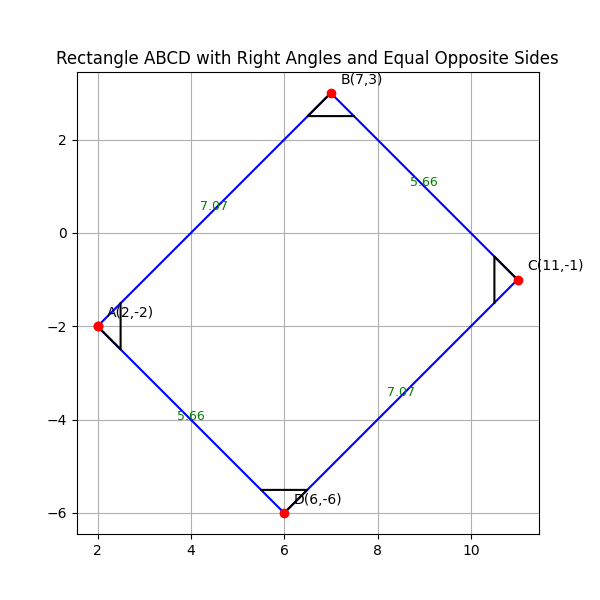
\includegraphics[width=0.6\columnwidth]{figs/1.png} 
    \caption{Plot for 2.4.34}
    \label{fig:placeholder}
\end{figure}
\end{frame}
\end{document}